% Options for packages loaded elsewhere
\PassOptionsToPackage{unicode}{hyperref}
\PassOptionsToPackage{hyphens}{url}
%
\documentclass[
]{article}
\usepackage{amsmath,amssymb}
\usepackage{lmodern}
\usepackage{iftex}
\ifPDFTeX
  \usepackage[T1]{fontenc}
  \usepackage[utf8]{inputenc}
  \usepackage{textcomp} % provide euro and other symbols
\else % if luatex or xetex
  \usepackage{unicode-math}
  \defaultfontfeatures{Scale=MatchLowercase}
  \defaultfontfeatures[\rmfamily]{Ligatures=TeX,Scale=1}
\fi
% Use upquote if available, for straight quotes in verbatim environments
\IfFileExists{upquote.sty}{\usepackage{upquote}}{}
\IfFileExists{microtype.sty}{% use microtype if available
  \usepackage[]{microtype}
  \UseMicrotypeSet[protrusion]{basicmath} % disable protrusion for tt fonts
}{}
\makeatletter
\@ifundefined{KOMAClassName}{% if non-KOMA class
  \IfFileExists{parskip.sty}{%
    \usepackage{parskip}
  }{% else
    \setlength{\parindent}{0pt}
    \setlength{\parskip}{6pt plus 2pt minus 1pt}}
}{% if KOMA class
  \KOMAoptions{parskip=half}}
\makeatother
\usepackage{xcolor}
\usepackage[margin=1in]{geometry}
\usepackage{color}
\usepackage{fancyvrb}
\newcommand{\VerbBar}{|}
\newcommand{\VERB}{\Verb[commandchars=\\\{\}]}
\DefineVerbatimEnvironment{Highlighting}{Verbatim}{commandchars=\\\{\}}
% Add ',fontsize=\small' for more characters per line
\usepackage{framed}
\definecolor{shadecolor}{RGB}{248,248,248}
\newenvironment{Shaded}{\begin{snugshade}}{\end{snugshade}}
\newcommand{\AlertTok}[1]{\textcolor[rgb]{0.94,0.16,0.16}{#1}}
\newcommand{\AnnotationTok}[1]{\textcolor[rgb]{0.56,0.35,0.01}{\textbf{\textit{#1}}}}
\newcommand{\AttributeTok}[1]{\textcolor[rgb]{0.77,0.63,0.00}{#1}}
\newcommand{\BaseNTok}[1]{\textcolor[rgb]{0.00,0.00,0.81}{#1}}
\newcommand{\BuiltInTok}[1]{#1}
\newcommand{\CharTok}[1]{\textcolor[rgb]{0.31,0.60,0.02}{#1}}
\newcommand{\CommentTok}[1]{\textcolor[rgb]{0.56,0.35,0.01}{\textit{#1}}}
\newcommand{\CommentVarTok}[1]{\textcolor[rgb]{0.56,0.35,0.01}{\textbf{\textit{#1}}}}
\newcommand{\ConstantTok}[1]{\textcolor[rgb]{0.00,0.00,0.00}{#1}}
\newcommand{\ControlFlowTok}[1]{\textcolor[rgb]{0.13,0.29,0.53}{\textbf{#1}}}
\newcommand{\DataTypeTok}[1]{\textcolor[rgb]{0.13,0.29,0.53}{#1}}
\newcommand{\DecValTok}[1]{\textcolor[rgb]{0.00,0.00,0.81}{#1}}
\newcommand{\DocumentationTok}[1]{\textcolor[rgb]{0.56,0.35,0.01}{\textbf{\textit{#1}}}}
\newcommand{\ErrorTok}[1]{\textcolor[rgb]{0.64,0.00,0.00}{\textbf{#1}}}
\newcommand{\ExtensionTok}[1]{#1}
\newcommand{\FloatTok}[1]{\textcolor[rgb]{0.00,0.00,0.81}{#1}}
\newcommand{\FunctionTok}[1]{\textcolor[rgb]{0.00,0.00,0.00}{#1}}
\newcommand{\ImportTok}[1]{#1}
\newcommand{\InformationTok}[1]{\textcolor[rgb]{0.56,0.35,0.01}{\textbf{\textit{#1}}}}
\newcommand{\KeywordTok}[1]{\textcolor[rgb]{0.13,0.29,0.53}{\textbf{#1}}}
\newcommand{\NormalTok}[1]{#1}
\newcommand{\OperatorTok}[1]{\textcolor[rgb]{0.81,0.36,0.00}{\textbf{#1}}}
\newcommand{\OtherTok}[1]{\textcolor[rgb]{0.56,0.35,0.01}{#1}}
\newcommand{\PreprocessorTok}[1]{\textcolor[rgb]{0.56,0.35,0.01}{\textit{#1}}}
\newcommand{\RegionMarkerTok}[1]{#1}
\newcommand{\SpecialCharTok}[1]{\textcolor[rgb]{0.00,0.00,0.00}{#1}}
\newcommand{\SpecialStringTok}[1]{\textcolor[rgb]{0.31,0.60,0.02}{#1}}
\newcommand{\StringTok}[1]{\textcolor[rgb]{0.31,0.60,0.02}{#1}}
\newcommand{\VariableTok}[1]{\textcolor[rgb]{0.00,0.00,0.00}{#1}}
\newcommand{\VerbatimStringTok}[1]{\textcolor[rgb]{0.31,0.60,0.02}{#1}}
\newcommand{\WarningTok}[1]{\textcolor[rgb]{0.56,0.35,0.01}{\textbf{\textit{#1}}}}
\usepackage{graphicx}
\makeatletter
\def\maxwidth{\ifdim\Gin@nat@width>\linewidth\linewidth\else\Gin@nat@width\fi}
\def\maxheight{\ifdim\Gin@nat@height>\textheight\textheight\else\Gin@nat@height\fi}
\makeatother
% Scale images if necessary, so that they will not overflow the page
% margins by default, and it is still possible to overwrite the defaults
% using explicit options in \includegraphics[width, height, ...]{}
\setkeys{Gin}{width=\maxwidth,height=\maxheight,keepaspectratio}
% Set default figure placement to htbp
\makeatletter
\def\fps@figure{htbp}
\makeatother
\setlength{\emergencystretch}{3em} % prevent overfull lines
\providecommand{\tightlist}{%
  \setlength{\itemsep}{0pt}\setlength{\parskip}{0pt}}
\setcounter{secnumdepth}{-\maxdimen} % remove section numbering
\newlength{\cslhangindent}
\setlength{\cslhangindent}{1.5em}
\newlength{\csllabelwidth}
\setlength{\csllabelwidth}{3em}
\newlength{\cslentryspacingunit} % times entry-spacing
\setlength{\cslentryspacingunit}{\parskip}
\newenvironment{CSLReferences}[2] % #1 hanging-ident, #2 entry spacing
 {% don't indent paragraphs
  \setlength{\parindent}{0pt}
  % turn on hanging indent if param 1 is 1
  \ifodd #1
  \let\oldpar\par
  \def\par{\hangindent=\cslhangindent\oldpar}
  \fi
  % set entry spacing
  \setlength{\parskip}{#2\cslentryspacingunit}
 }%
 {}
\usepackage{calc}
\newcommand{\CSLBlock}[1]{#1\hfill\break}
\newcommand{\CSLLeftMargin}[1]{\parbox[t]{\csllabelwidth}{#1}}
\newcommand{\CSLRightInline}[1]{\parbox[t]{\linewidth - \csllabelwidth}{#1}\break}
\newcommand{\CSLIndent}[1]{\hspace{\cslhangindent}#1}
\ifLuaTeX
  \usepackage{selnolig}  % disable illegal ligatures
\fi
\IfFileExists{bookmark.sty}{\usepackage{bookmark}}{\usepackage{hyperref}}
\IfFileExists{xurl.sty}{\usepackage{xurl}}{} % add URL line breaks if available
\urlstyle{same} % disable monospaced font for URLs
\hypersetup{
  pdftitle={Check your outliers! An accessible introduction to identifying statistical outliers with R and easystats},
  hidelinks,
  pdfcreator={LaTeX via pandoc}}

\title{Check your outliers! An accessible introduction to identifying
statistical outliers with R and \emph{easystats}}
\usepackage{etoolbox}
\makeatletter
\providecommand{\subtitle}[1]{% add subtitle to \maketitle
  \apptocmd{\@title}{\par {\large #1 \par}}{}{}
}
\makeatother
\subtitle{(Alt title:) Statistical Outliers: Univariate, Multivariate,
and Model-Based}
\author{}
\date{\vspace{-2.5em}}

\begin{document}
\maketitle

\hypertarget{abstract}{%
\section{Abstract}\label{abstract}}

xyz

\hypertarget{introduction}{%
\section{Introduction}\label{introduction}}

Statistical outliers need to be addressed because they can significantly
affect our statistical models.

Leys et al. (2019) distinguish between error outliers, interesting
outliers, and random outliers.

\hypertarget{current-recommendations}{%
\subsection{Current recommendations}\label{current-recommendations}}

Current guidelines recommend the following:

We note also that ideally the handling of outliers should be
preregistered a priori (Leys et al., 2019).

\hypertarget{univariate-outliers}{%
\section{Univariate Outliers}\label{univariate-outliers}}

When using t-tests for example.

For univariate outliers, it is recommended (Leys et al., 2013, 2019) to
use the Median Absolute Deviation (MAD). In easystats'
\texttt{check\_outliers()},one can use this approach with
\texttt{method\ =\ "zscore\_robust"}.

Example:

\begin{Shaded}
\begin{Highlighting}[]
\FunctionTok{library}\NormalTok{(performance)}
\NormalTok{data }\OtherTok{\textless{}{-}} \FunctionTok{na.omit}\NormalTok{(airquality)}

\NormalTok{x }\OtherTok{\textless{}{-}} \FunctionTok{check\_outliers}\NormalTok{(data, }\AttributeTok{method =} \StringTok{"zscore\_robust"}\NormalTok{)}
\NormalTok{x}
\end{Highlighting}
\end{Shaded}

\begin{verbatim}
## 7 outliers detected: cases 23, 30, 34, 63, 65, 77, 80.
## - Based on the following method and threshold: zscore_robust (3.09).
## - For variables: Ozone, Solar.R, Wind, Temp, Month, Day.
## 
## -----------------------------------------------------------------------------
## Outliers per variable (zscore_robust): 
## 
## $Ozone
##    Row Distance_Zscore_robust
## 23  23               3.332778
## 34  34               4.126296
## 63  63               3.610509
## 65  65               3.134398
## 77  77               5.435602
## 80  80               3.451806
## 
## $Wind
##    Row Distance_Zscore_robust
## 30  30               3.225825
\end{verbatim}

\begin{Shaded}
\begin{Highlighting}[]
\FunctionTok{library}\NormalTok{(see)}
\FunctionTok{plot}\NormalTok{(x)}
\end{Highlighting}
\end{Shaded}

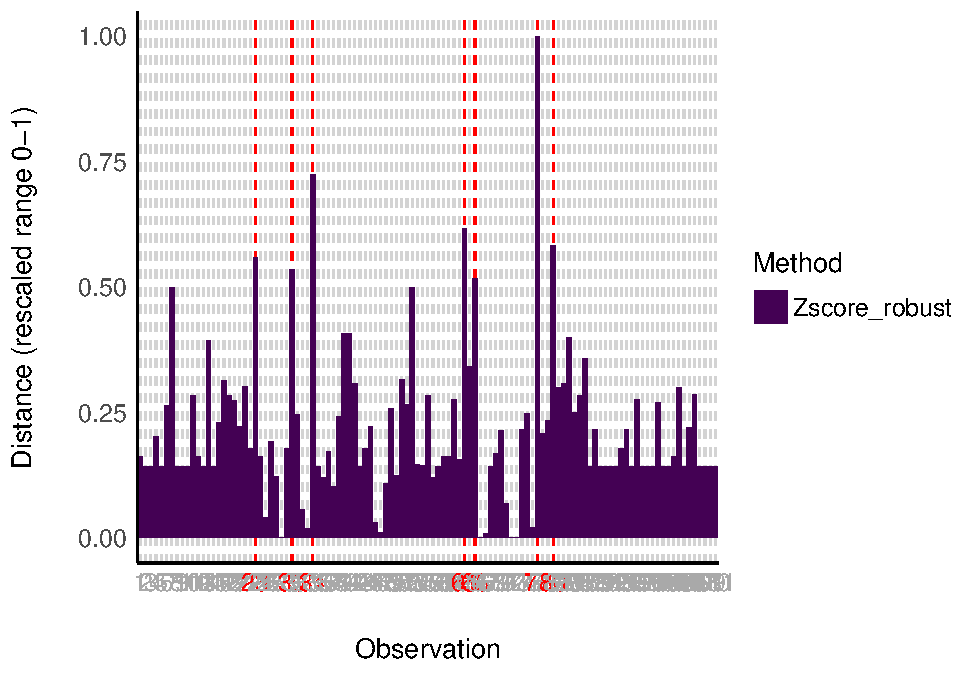
\includegraphics{paper_files/figure-latex/univariate outliers-1.pdf}

\hypertarget{multivariate-outliers}{%
\section{Multivariate Outliers}\label{multivariate-outliers}}

For multivariate outliers, it is recommended (Leys et al., 2019) to use
the Minimum Covariance Determinant (MCD).

Example:

\begin{Shaded}
\begin{Highlighting}[]
\NormalTok{x }\OtherTok{\textless{}{-}} \FunctionTok{check\_outliers}\NormalTok{(data, }\AttributeTok{method =} \StringTok{"mcd"}\NormalTok{)}
\NormalTok{x}
\end{Highlighting}
\end{Shaded}

\begin{verbatim}
## 12 outliers detected: cases 1, 4, 6, 7, 11, 14, 17, 19, 20, 23, 34, 77.
## - Based on the following method and threshold: mcd (22.46).
## - For variables: Ozone, Solar.R, Wind, Temp, Month, Day.
\end{verbatim}

\begin{Shaded}
\begin{Highlighting}[]
\FunctionTok{plot}\NormalTok{(x)}
\end{Highlighting}
\end{Shaded}

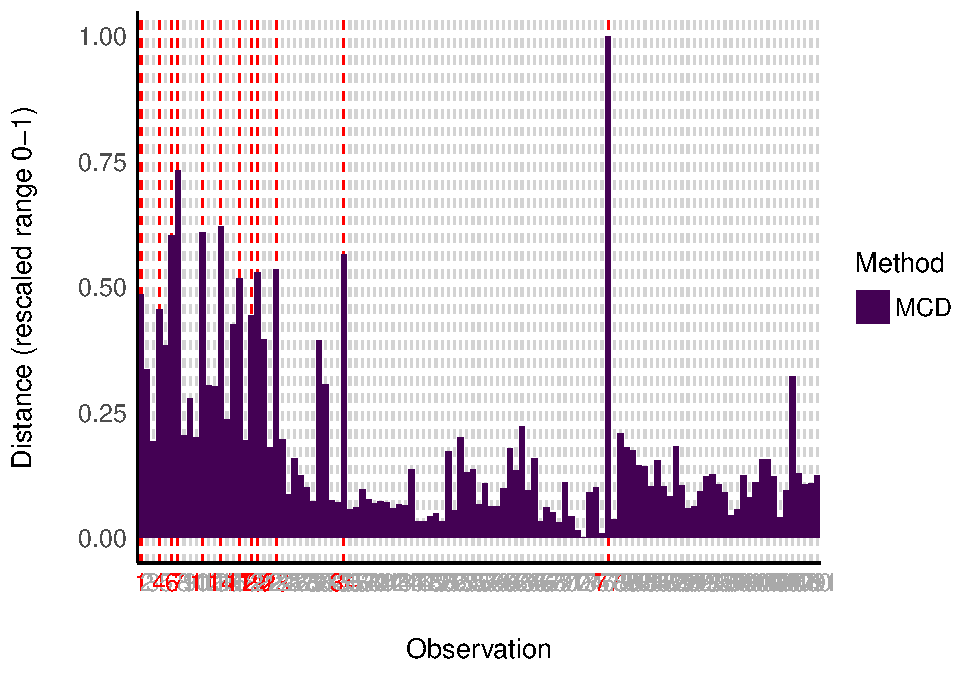
\includegraphics{paper_files/figure-latex/multivarite outliers-1.pdf}

\hypertarget{model-based-outliers}{%
\section{Model-Based Outliers}\label{model-based-outliers}}

When using linear regression models for example.

Example:

\begin{Shaded}
\begin{Highlighting}[]
\CommentTok{\# create some fake outliers}
\NormalTok{data }\OtherTok{\textless{}{-}} \FunctionTok{rbind}\NormalTok{(mtcars, }\DecValTok{42}\NormalTok{, }\DecValTok{55}\NormalTok{)}

\CommentTok{\# fit model with outliers}
\NormalTok{model }\OtherTok{\textless{}{-}} \FunctionTok{lm}\NormalTok{(disp }\SpecialCharTok{\textasciitilde{}}\NormalTok{ mpg }\SpecialCharTok{+}\NormalTok{ hp, }\AttributeTok{data =}\NormalTok{ data)}
\NormalTok{x }\OtherTok{\textless{}{-}} \FunctionTok{check\_outliers}\NormalTok{(model, }\AttributeTok{method =} \StringTok{"cook"}\NormalTok{)}
\NormalTok{x}
\end{Highlighting}
\end{Shaded}

\begin{verbatim}
## 2 outliers detected: cases 31, 34.
## - Based on the following method and threshold: cook (0.81).
## - For variable: (Whole model).
\end{verbatim}

\begin{Shaded}
\begin{Highlighting}[]
\FunctionTok{plot}\NormalTok{(x)}
\end{Highlighting}
\end{Shaded}

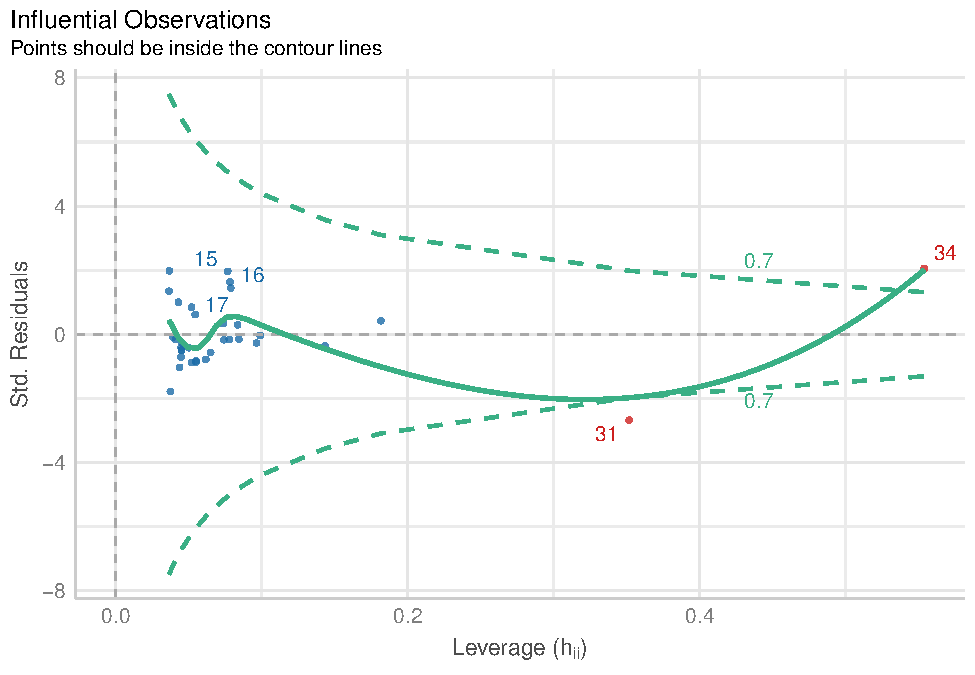
\includegraphics{paper_files/figure-latex/model-based outliers-1.pdf}

\hypertarget{multiple-methods}{%
\section{Multiple methods}\label{multiple-methods}}

An alternative approach suggested by easystats is to combine several
methods (model-based, univariate, and multivariate). This approach
computes a composite outlier score, made of the average of the binary (0
or 1) results of each method. It represents the probability of each
observation to be classified as an outlier by at least one method. The
default decision rule classifies rows with composite outlier scores
superior or equal to 0.5 as outlier observations (i.e., that were
classified as outliers by at least half of the methods).

Example:

\begin{Shaded}
\begin{Highlighting}[]
\NormalTok{x }\OtherTok{\textless{}{-}} \FunctionTok{check\_outliers}\NormalTok{(data, }\AttributeTok{method =} \FunctionTok{c}\NormalTok{(}
  \StringTok{"zscore"}\NormalTok{, }\StringTok{"IQR"}\NormalTok{, }\StringTok{"mahalanobis"}\NormalTok{, }\StringTok{"mahalanobis\_robust"}\NormalTok{, }\StringTok{"mcd"}\NormalTok{, }\StringTok{"ics"}\NormalTok{, }\StringTok{"optics"}\NormalTok{, }\StringTok{"lof"}\NormalTok{))}
\NormalTok{x}
\end{Highlighting}
\end{Shaded}

\begin{verbatim}
## 2 outliers detected: cases 33, 34.
## - Based on the following methods and thresholds: zscore (3.09),
##   mahalanobis (31.26), mahalanobis_robust (31.26), mcd (31.26), ics
##   (0.001), optics (22), lof (0.001).
## - For variables: mpg, cyl, disp, hp, drat, wt, qsec, vs, am, gear, carb.
## Note: Outliers were classified as such by at least half of the selected methods. 
## 
## -----------------------------------------------------------------------------
## The following observations were considered outliers for two or more variables 
## by at least one of the selected methods: 
## 
##    Row n_Zscore n_Mahalanobis_robust          n_MCD          n_ICS
## 1   34        9       (Multivariate) (Multivariate) (Multivariate)
## 2   33        7       (Multivariate) (Multivariate) (Multivariate)
## 3    9        0       (Multivariate) (Multivariate)              0
## 4   19        0       (Multivariate)              0              0
## 5   27        0       (Multivariate) (Multivariate)              0
## 6   28        0       (Multivariate) (Multivariate)              0
## 7   29        0       (Multivariate)              0              0
## 8   30        0       (Multivariate) (Multivariate)              0
## 9   31        0       (Multivariate) (Multivariate) (Multivariate)
## 10   8        0                    0 (Multivariate)              0
## 11  21        0                    0 (Multivariate)              0
##             n_LOF
## 1  (Multivariate)
## 2  (Multivariate)
## 3               0
## 4               0
## 5               0
## 6               0
## 7               0
## 8               0
## 9               0
## 10              0
## 11              0
\end{verbatim}

An example sentence for reporting the usage of the composite method
could be:

\begin{quote}
Based on a composite outlier score (see the `check\_outliers' function
in the `performance' R package; Lüdecke et al., 2021) obtained via the
joint application of multiple outliers detection algorithms (Z-scores,
Iglewicz, 1993; Interquartile range (IQR); Mahalanobis distance, Cabana,
2019; Robust Mahalanobis distance, Gnanadesikan and Kettenring, 1972;
Minimum Covariance Determinant, Leys et al., 2018; Invariant Coordinate
Selection, Archimbaud et al., 2018; OPTICS, Ankerst et al., 1999;
Isolation Forest, Liu et al.~2008; and Local Outlier Factor, Breunig et
al., 2000), we excluded one participant that was classified as outlier
by at least half of the methods used.
\end{quote}

\hypertarget{conclusion}{%
\section{Conclusion}\label{conclusion}}

This is the conclusion.

\hypertarget{references}{%
\section*{References}\label{references}}
\addcontentsline{toc}{section}{References}

\hypertarget{refs}{}
\begin{CSLReferences}{1}{0}
\leavevmode\vadjust pre{\hypertarget{ref-leys2019outliers}{}}%
Leys, C., Delacre, M., Mora, Y. L., Lakens, D., \& Ley, C. (2019). How
to classify, detect, and manage univariate and multivariate outliers,
with emphasis on pre-registration. \emph{International Review of Social
Psychology}. \url{https://doi.org/10.5334/irsp.289}

\leavevmode\vadjust pre{\hypertarget{ref-leys2013outliers}{}}%
Leys, C., Ley, C., Klein, O., Bernard, P., \& Licata, L. (2013).
Detecting outliers: Do not use standard deviation around the mean, use
absolute deviation around the median. \emph{Journal of Experimental
Social Psychology}, \emph{49}(4), 764--766.
https://doi.org/\url{https://doi.org/10.1016/j.jesp.2013.03.013}

\end{CSLReferences}

\end{document}
